%<dscrpt>Suite de nombres complexes modélisant un billard.</dscrpt>
Dans un plan horizontal, on considère un billard circulaire \footnote{d'après X 98 PC 1} de rayon 1. Il est identifié au disque unité du plan complexe et son bord au cercle unité $\U$ de centre 0.
\begin{displaymath}
  D=\{z\in \C, |z|\leq 1\} \hspace{1cm} \U =\{z\in \C, |z|= 1\}
\end{displaymath}
Une boule (ponctuelle) est lancée à l'instant $t=0$ d'un point $M_0$ (d'affixe $z_0$) du bord. Elle rebondit contre le bord du billard en des points $M_1, M_2, \cdots, M_i, \cdots$ d'affixes $z_1, z_2, \cdots, z_i,\cdots$.\newline
On suppose que son mouvement est rectiligne uniforme (norme de la vitesse égale 1) entre deux chocs et qu'il se poursuit indéfiniment. Les vitesses entre $M_0, M_1, M_2, \cdots$ sont notées $\overrightarrow{v_0}, \overrightarrow{v_1}, \overrightarrow{v_2}, \cdots$. Elles sont de norme $1$ et d'affixes $v_0, v_1, v_2, \cdots$.\newline
Les chocs sont des \emph{réflexions élastiques}; c'est à dire que la normale en un point du bord du billard où un choc se produit est la bissectrice intérieure de deux segments de trajectoire consécutifs.\newline
\begin{figure}[h]
\centering
  \subfloat[Choc élastique en $M_k$]{\label{fig:Ebillard_1} 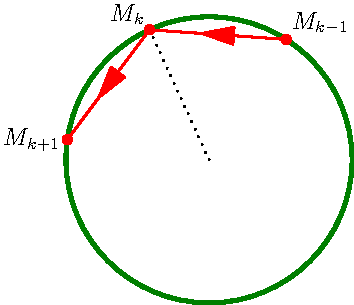
\includegraphics[width=5cm]{./Ebillard_1.pdf}} \hspace{1cm}
  \subfloat[Vitesse initiale]{\label{fig:Ebillard_2} 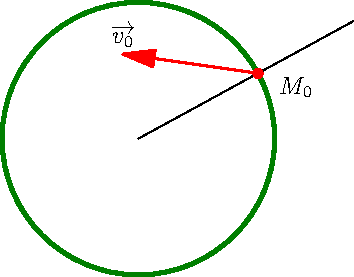
\includegraphics[width=5cm]{./Ebillard_2.pdf}}
\caption{Billard}
\end{figure}
On écrit l'affixe de la vitesse initiale sous la forme $v_0 = z_0e^{i\alpha}$ avec $\alpha \in [0,2\pi[$.
\begin{enumerate}
  \item Quel angle représente $\alpha$? Dans quel intervalle doit-il se trouver ? 
  \item Simplifier $1-2\cos\alpha e^{i\alpha}$ sous la forme d'une seule exponentielle.
  \item Calcul de $M_1$.
  \begin{enumerate}
\item Préciser géométriquement l'ensemble des points $P$ d'affixe $w$ vérifiant:
\begin{displaymath}
  \exists \lambda \in \R \text{ tel que } w = z_0 + \lambda v_0
\end{displaymath}
\item Calculer l'affixe $z_1$ du point $M_1$ du bord en lequel se produit le premier choc. Donner un argument de $\frac{v_0}{z_1}$.
\end{enumerate}

\item Calcul de $\overrightarrow{v_1}$. \label{tradrefl}Traduire la propriété de réflexion élastique en $M_1$ par une relation entre des arguments de $\frac{v_0}{z_1}$ et de $\frac{v_1}{z_1}$. En déduire $\frac{v_1}{z_1}$.

\item \label{relfond} Montrer qu'il existe $\beta \in ]0,2\pi[$ indépendant de $n$ (à exprimer avec $\alpha$) tel que :
\begin{displaymath}
 \forall n\in \N^{*}, \;z_n = z_0 e^{in\beta}
\end{displaymath}

\item Quelle est la longueur d'une corde $M_{j-1}M_{j}$ pour $j\in \N^{*}$ ?

\item Donner une condition nécessaire et suffisante sur $\alpha$ pour que le mouvement soit périodique. Préciser la période et la trajectoire.

\item Autre méthode pour les résultats des questions \ref{tradrefl} et \ref{relfond}.\newline
En exploitant symétrie et rotation, former une relation entre $\frac{z_{k+1}}{z_k}$ et $\frac{z_{k-1}}{z_k}$. En déduire une expression de $z_{k+1}$ en fonction de $z_k$ et $z_{k-1}$.\newline
Que devient cette relation si $z_k=e^{i\beta}z_{k-1}$? Conclure.  
\end{enumerate}

